\section{Технический проект}
\subsection{Общая характеристика организации решения задачи}

Целью этого проекта является спроектировать и разработать приложение, которое поможет специализированным службам по тушению всеразличных возгораний вести более эффективную и проработанную деятельность.

Это приложение представляет собой интеллектуальную систему, предназначеную для автоматического обнаружения и классификации очагов возгораний. Эта система способна, при помощи нейронной сети, распознавать объекты, такие как возгорания и пожары, и определять их класс и уровень опасности на основе цветовых характеристик и наличиии задымленности на изображении, а также обучаться при помощи пользователя.

\subsection{Обоснование выбора технологии проектирования}

Для задачи классификации возгораний, полученных с БПЛА, используется две сверточных нейроных сетей. Такие сети хорошо подходят для задачи обработки изображений и классификации объектов, что делает их эффективным выбором для анализа данных с камер БПЛА. Она способна извлекать характерные признаки из изображений, таких как формы, текстуры и цвета, что позволяет эффективно классифицировать возгорания.

\subsubsection{Описание используемых технологий и языков программирования}

В процессе разработки приложения используются программные средства и языки программирования. Каждое программное средство и каждый язык программирования применяется для круга задач, при решении которых они необходимы.

\subsubsection{Сверточные нейронные сети}

Convolutional neural network(CNN) или Сверточная нейронная сеть - это тип искусственной нейронной сети, который широко используется для задач обработки изображений и компьютерного зрения. Ключевой особенностью CNN является использование сверточных слоев, которые извлекают характерные признаки из входных изображений. Эти признаки могут включать в себя формы, текстуры, края или цвета.

Основная идея CNN заключается в применении сверточных фильтров к входному изображению, что позволяет выявить повторяющиеся шаблоны или признаки. Эти фильтры скользят по изображению, извлекая информацию на разных уровнях абстракции. Затем эта информация проходит через дополнительные слои, такие как подвыборка или пулинг, которые уменьшают пространственные размеры данных, и полностью подключенные слои, которые выполняют классификацию или регрессию.

CNN показали впечатляющие результаты в задачах классификации изображений, обнаружения объектов, сегментации и даже в анализе медицинских изображений. Они эффективно обрабатывают большие объемы данных, обучаясь выявлять сложные зависимости и характерные признаки.

\subsubsection{Машинное обучение}

Машинное обучение - это раздел искусственного интеллекта, который фокусируется на разработке алгоритмов и моделей, позволяющих компьютерам обучаться и улучшать свои задачи без явного программирования.

Применение алгоритмов машинного обучения лежит в основе нашей системы анализа и классификации данных. Мы обучаем нашу модель на обширной базе изображений, позволяя системе эффективно распознавать и классифицировать объекты в реальном времени. Этот процесс включает в себя использование сложных алгоритмов, которые могут извлекать и интерпретировать характерные особенности из данных изображений.

\subsubsection{Язык программирования Python}

Python является одним из самых популярных и широко используемых языков программирования для разработки приложений искусственного интеллекта и машинного обучения. Он имеет простой и понятный синтаксис, что ускоряет процесс разработки и делает код более читаемым.

\subsubsection{Библиотеки Python}
Библиотеки, использованные в нашей программе:
\begin{enumerate}
\item NumPy. Фундаментальная библиотека для научных расчетов в Python. Она обеспечивает эффективную работу с многомерными массивами и матричными вычислениями, что критически важно для обработки и манипуляции данными.
\item Matplotlib. Библиотека для визуализации данных. Она позволяет создавать настраиваемые и интуитивно понятные графики, диаграммы и изображения, что облегчает визуальный анализ данных и представление результатов.
\item OpenCV (Open Source Computer Vision Library). Библиотека компьютерного зрения, которая предлагает широкий спектр алгоритмов для обработки изображений и видео. Она идеально подходит для задач обработки изображений, обнаружения объектов и анализа видео, полученных с камер БПЛА.
\item Pandas. Библиотека для анализа и манипуляции данными. Она предоставляет удобные структуры данных, такие как DataFrame, и богатый набор инструментов для обработки, фильтрации и агрегации данных, упрощая подготовку и анализ больших наборов данных.
\item TensorFlow. Это открытая платформа машинного обучения с масштабируемыми инструментами для обучения и развертывания моделей. Она обеспечивает гибкую и эффективную инфраструктуру для создания сложных нейронных сетей. Keras - это высокоуровневый API, построенный на TensorFlow, который упрощает процесс создания и обучения нейронных сетей. Он предлагает простой и интуитивно понятный интерфейс, позволяя быстро разрабатывать и экспериментировать с различными архитектурами моделей.
\end{enumerate}

\subsubsection{Архитектура сверточной нейронной сети}

Архитектура сверточной нейронной сети включает в себя 14 слоев с различными функциями.

Схема архитектуры нейронной сети представлена на рисунке ~\ref{archNC:image}.

\begin{figure}[H]
\center{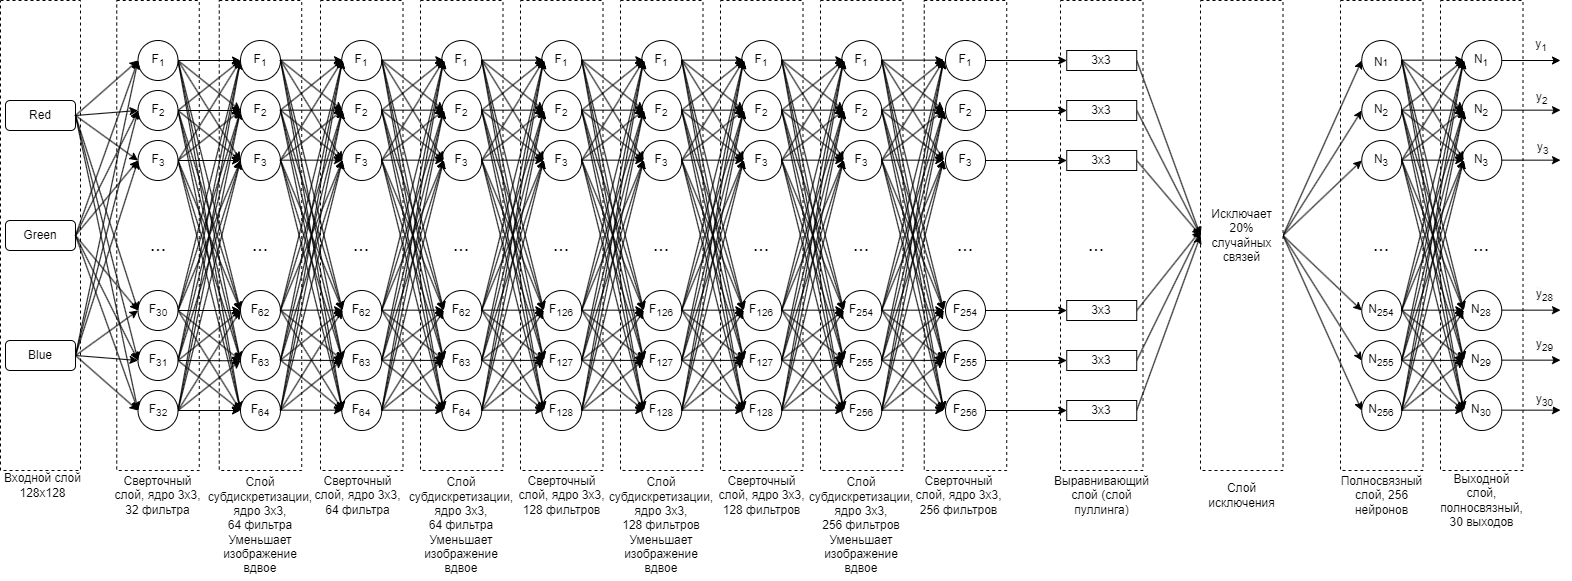
\includegraphics[width=1\linewidth]{archNC}}
\caption{Архитектура нейронной сети}
\label{archNC:image}
\end{figure}

Слои нейронной сети классификации описаны далее:

\begin{enumerate}
\item Input Layer (Входной слой).

Функция Input определяет входной слой с размером изображения 128×128 пикселей и 3 цветовыми каналами (RGB).
\item Convolutional Layers (Сверточные слои, 9).

Первый свёрточный слой Conv2D имеет 32 фильтра размером 3×3, функцию активации ReLU и параметр padding='same', который сохраняет размерность входного изображения.

Второй свёрточный слой Conv2D увеличивает количество фильтров до 64 и применяет шаг (strides) равный 2, что уменьшает размерность изображения вдвое.

Следующие два слоя Conv2D также имеют 64 фильтра и один из них снова применяет шаг 2 для уменьшения размерности.

Пятый и шестой свёрточные слои Conv2D содержат 128 фильтров каждый, с шагом 2 на шестом слое.

Седьмой свёрточный слой Conv2D сохраняет 128 фильтров и размерность.

Восьмой и девятый свёрточные слои Conv2D увеличивают количество фильтров до 256, с шагом 2 на восьмом слое.
\item Flatten Layer (Выравнивающий слой).

Слой Flatten преобразует многомерный тензор свёрточных слоёв в одномерный, чтобы его можно было подать на полносвязные слои.
\item Dropout Layer (Слой исключения).

Слой Dropout с параметром 0.2 предотвращает переобучение, случайным образом "выключая" 20\% нейронов на каждом шаге обучения.
\item Dense Layers (Полносвязные слои, 2).

Первый полносвязный слой Dense имеет 256 нейронов и функцию активации ReLU.

Второй полносвязный слой Dense формирует выходной слой с 30 нейронами, количество которых соответствует количеству выходных значений, которые должна предсказывать модель.
\end{enumerate}

\subsubsection{Функция активации ReLU}

ReLU, или Rectified Linear Unit, — это функция активации, которая используется в нейронных сетях для увеличения нелинейности. 
Формула ReLU предоставлена формулой ~\ref{form0:equation}.

\begin{equation}
    \fontsize{17}{20}{f(x)=max(0,x)}
    \label{form0:equation}
\end{equation}

Это означает, что если вход x положительный, то функция возвращает x, а если x отрицательный, то функция возвращает 0. 
ReLU популярна потому, что она ускоряет обучение нейронных сетей без значительной потери точности. Она также помогает решить проблему исчезающего градиента, так как производная для положительных значений всегда равна 1, что обеспечивает более быстрое и эффективное обучение.

График функции ReLu предоставлен на изображении  ~\ref{relu:image}.

\begin{figure}[H]
\center{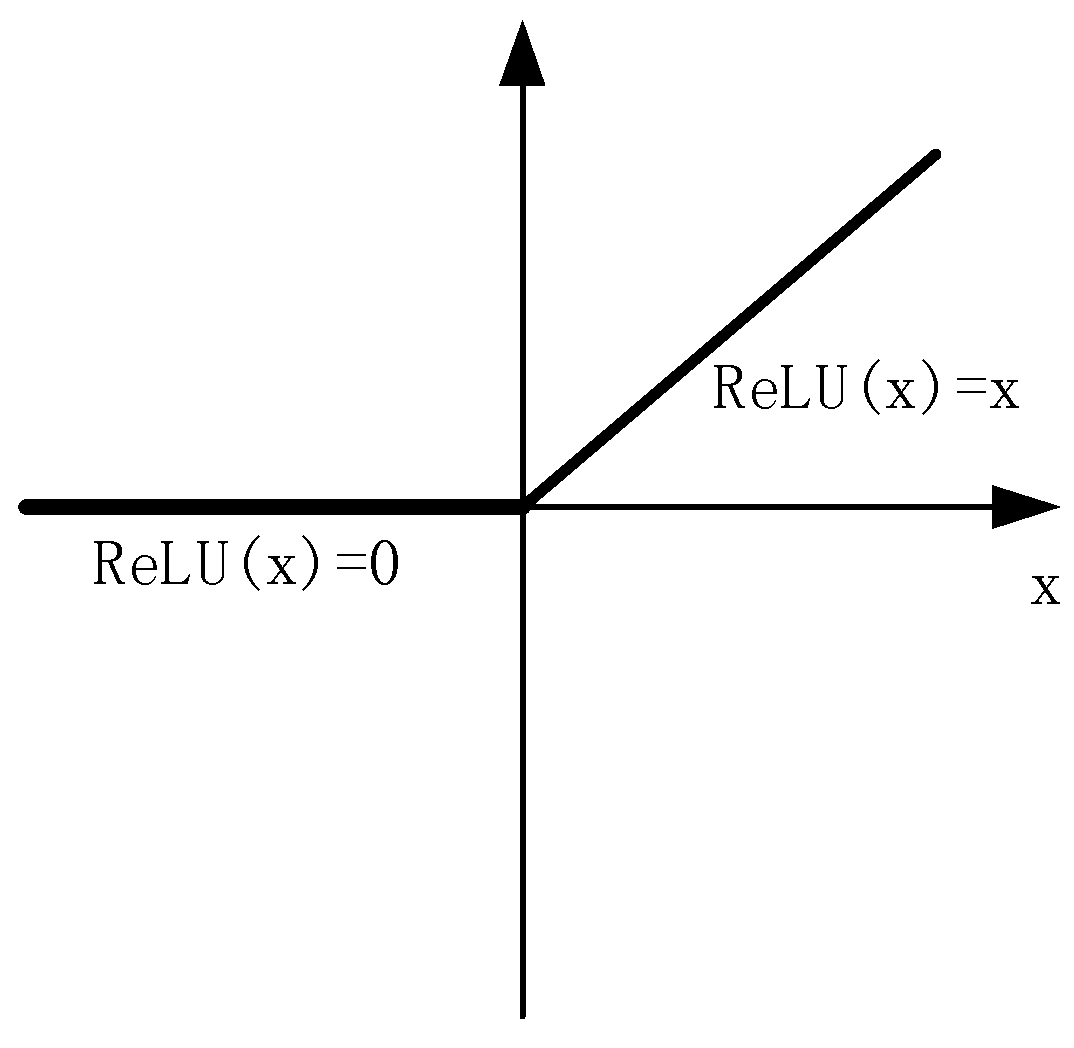
\includegraphics[width=1\linewidth]{relu}}
\caption{График функции ReLU}
\label{relu:image}
\end{figure}

\subsubsection{Функция IoU Loss}
Intersection over Union (IoU) является метрикой, используемой для измерения точности объектного детектора на определенном наборе данных. Если мы работаем с задачами компьютерного зрения, такими как сегментация изображений или обнаружение объектов, IoU может помочь оценить, насколько предсказанные границы объекта соответствуют истинным границам.

Наглядным образом функцию можно увидеть на изображении ~\ref{iou:image}.

\begin{figure}[H]
\center{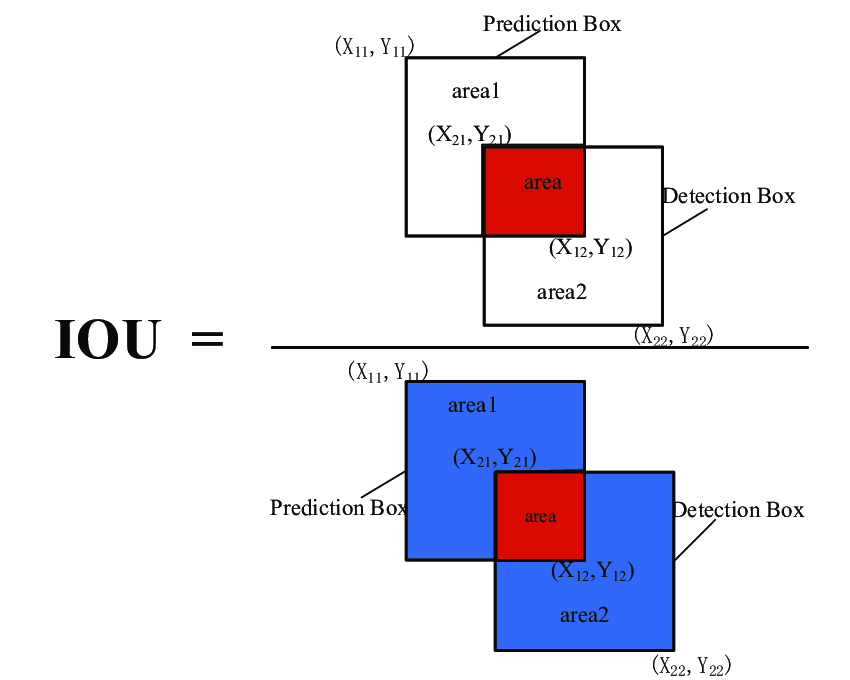
\includegraphics[width=1\linewidth]{iou}}
\caption{График функции IoU}
\label{iou:image}
\end{figure}

IoU рассчитывается по формуле ~\ref{form1:equation}.

\begin{equation}
    \fontsize{17}{20}{IoU= \frac{\text{площадь объединения}}{\text{площадь пересечения}}}
    \label{form1:equation}
\end{equation}

Где:
\begin{itemize}
\item площадь пересечения - это область, где предсказанная граница и истинная граница объекта перекрываются;
\item площадь объединения - это область, покрытая как предсказанной границей, так и истинной границей, вместе взятых.
\end{itemize}

IoU loss - это функция потерь, которая используется для обучения моделей, выполняющих задачи, связанные с локализацией объектов. Вместо того чтобы использовать стандартные функции потерь, такие как кросс-энтропия, которые могут не полностью отражать точность локализации, IoU loss напрямую оптимизирует метрику IoU, стремясь увеличить площадь пересечения и уменьшить площадь объединения.

Функция потерь IoU показана в формуле ~\ref{form2:equation}.

\begin{equation}
	\fontsize{17}{20}{IoU loss=1−IoU}
	\label{form2:equation}
\end{equation}

Таким образом, минимизация IoU loss в процессе обучения приводит к увеличению IoU между предсказанными и истинными границами, что помогает в задаеч локализации объектов нашего проекта.

\subsection{Диаграмма компонентов}

Диаграмма компонентов представляет структуру системы в виде набора компонентов и их взаимосвязей. Каждый компонент отвечает за определенную функцию в рамках системы и может включать в себя подсистемы или модули.
Компоненты программы:
\begin{enumerate}
\item Графический интерфейс. Отвечает за создание интерфейса, в котором пользователь наглядно видит результат распознования в сравнении с оригиналом.
\item Обработка изображения. Включает в себя методы улучшения качества изображений, такие как коррекция освещения, удаление шумов и извлечение важных признаков.
\item Сверточная нейронная сеть (CNN). Ядро этой системы, реализующее алгоритмы обучения и распознавания объектов.
\item Данные параметров нейронной сети. Представляют собой обученную модель, которая хранит в себе веса и параметры, извлеченные из данных во время процесса обучения.
\item Классификация объекта. Этот модуль используется для классификации возгорания.
\item Генерация отчета. Отвечает за создание отчета для выведения класса возгорания и оценки его опасности.
\end{enumerate}

\subsubsection{Взаимодействие компонентов}

Взаимодействие компонентов проходит по такой цепочке:
\begin{enumerate}
\item Пользователь загружает изображение через графический интерфейс пользователя.
\item Интерфейс передает изображение в модуль обработки изображения.
\item После обработки данные передаются в модуль сверточной нейронной сети для распознавания объекта.
\item Модуль данных параметров передает веса и параметры и корректирует работу нейронной сети.
\item Результаты распознавания классифицируются в модуле классификации объекта.
\item Модуль генерации отчета выводит данные о возгорании в графическом интерфейсе.
\end{enumerate}

Диаграмма компонентов представленна на рисунке ~\ref{comp:image}.

\begin{figure}[H]
\center{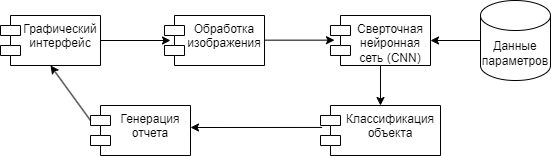
\includegraphics[width=1\linewidth]{comp}}
\caption{Диаграмма компонентов}
\label{comp:image}
\end{figure}

\subsubsection{Диаграмма программных классов}

Точкой входа в программу является класс main. В этом классе осуществляется запуск и инициализация основных компонентов программы:
\begin{itemize}
	\item dataprocessing -- компонент, отвечающий за обработку данных и изображений.
	\item creatingtfrecordclassifier -- компонент, отвечающий за создание и загрузку изображений и создания их записи в формате .tfrecord.
	\item creatingtfrecordlocalizer -- компонент, отвечающий за создание и загрузку изображений и создания их записи в формате .tfrecord.
	\item classifier -- компонент, отвечающий за работу с нейронной сетью по классификации данных, её обучение и тестирование.
	\item training -- компонент, отвечающий за работу с нейронной сетью по распознанию данных, её обучение и тестирование.
\end{itemize}

Диаграмма классов предоставлена на рисунке ~\ref{classdiag:image}.

\begin{figure}[H]
\center{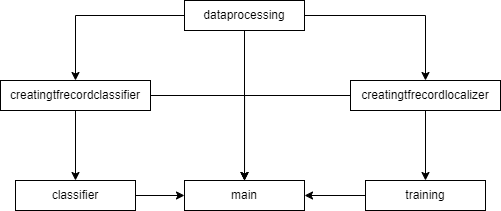
\includegraphics[width=1\linewidth]{classdiag}}
\caption{Диаграмма классов и их связей}
\label{classdiag:image}
\end{figure}

На диаграмме показаны данные связи:
\begin{enumerate}
	\item Связь dataprocessing - main. Класс main использует основные функции класса dataprocessing, такие как отображение информации о изображении, загрузка изображения и нормализация координат изображения.
	\item Связь dataprocessing - creatingtfrecordclassifier. Класс creatingtfrecordclassifier использует основные функции класса dataprocessing, такие как загрузка изображения и нормализация координат изображения. Для создания записи tfrecord необходимо создать запись со всеми изображениями и файлами формата .xml.
	\item Связь dataprocessing - creatingtfrecordlocalizer. Класс creatingtfrecordlocalizer использует основные функции класса dataprocessing, такие как загрузка изображения и нормализация координат изображения. Для создания записи tfrecord необходимо создать запись со всеми изображениями и файлами формата .xml.
	\item Связь creatingtfrecordclassifier - classifier. Для работы классу classifier нужен созданный в классе creatingtfrecordclassifier файл tfrecord.
	\item Связь creatingtfrecordclassifier - main.  Класс main использует основные функции класса creatingtfrecordclassifier, такие как создание файла tfrecord для классификатора.
	\item Связь creatingtfrecordlocalizer - training. Для работы классу training нужен созданный в классе creatingtfrecordlocalizer файл tfrecord.
	\item Связь creatingtfrecordlocalizer - main.  Класс main использует основные функции класса creatingtfrecordlocalizer, такие как создание файла tfrecord для локализатора.
	\item Связь classifier - main. Класс main использует основные функции класса classifier, такие как тестирование, обучение, загрузка и сохранение сети.
	\item Связь localizer - main. Класс main использует основные функции класса localizer, такие как тестирование, обучение, загрузка и сохранение сети.
\end{enumerate}


\subsection{ Проектирование пользовательского интерфейса}
На основании требований к пользовательскому интерфейсу, представленных в пункте 2.3 технического задания, был разработан графический интерфейс приложения. Для создания пользовательского интерфейса используется библеотека tkinter и matlibplot.

На рисунке ~\ref{maketinterface:image} представлен макет интерфейса окон для распознания и обучения нейронной сети. Данный макет содержит следующие элементы:
\begin{enumerate}
\item Загрузка изображения из системы.
\item Загрузка своей модели нейронной сети.
\item Запустить распознание изображения
\item Открыть окно тренировки модели нейронной сети.
\item Поле загруженного изображения.
\item Поле изображения с распознанным возгоранием.
\item Закрывает окно тренировки модели нейронной сети.
\item Показывает информацию о первой картинке в папке с изображениями для обучения.
\item Запускает стороннюю программу labelimg.
\item Показывает в поле для вывода информацию о наличии файлов.
\item Создает новую запись tfrecord для локализатора.
\item Создает новую запись tfrecord для классификатора.
\item Запускает функцию тестирования классификатора.
\item Запускает другую функцию тестриования классификатора с точными значениями.
\item Запускает функцию обучения классификатора.
\item Сохраняет модель нейронной сети классификатора.
\item Сохраняет модель нейронной сети локализатора.
\item Загружает модель нейронной сети локализатора.
\item Запускает функцию тестирования нейронной сети локализатора.
\item Запускает функции для обучения нейронной сети локализатора.
\item Поле вывода информации из терминала после выполнения любых операций.
\end{enumerate}

\begin{figure}[H]
\center{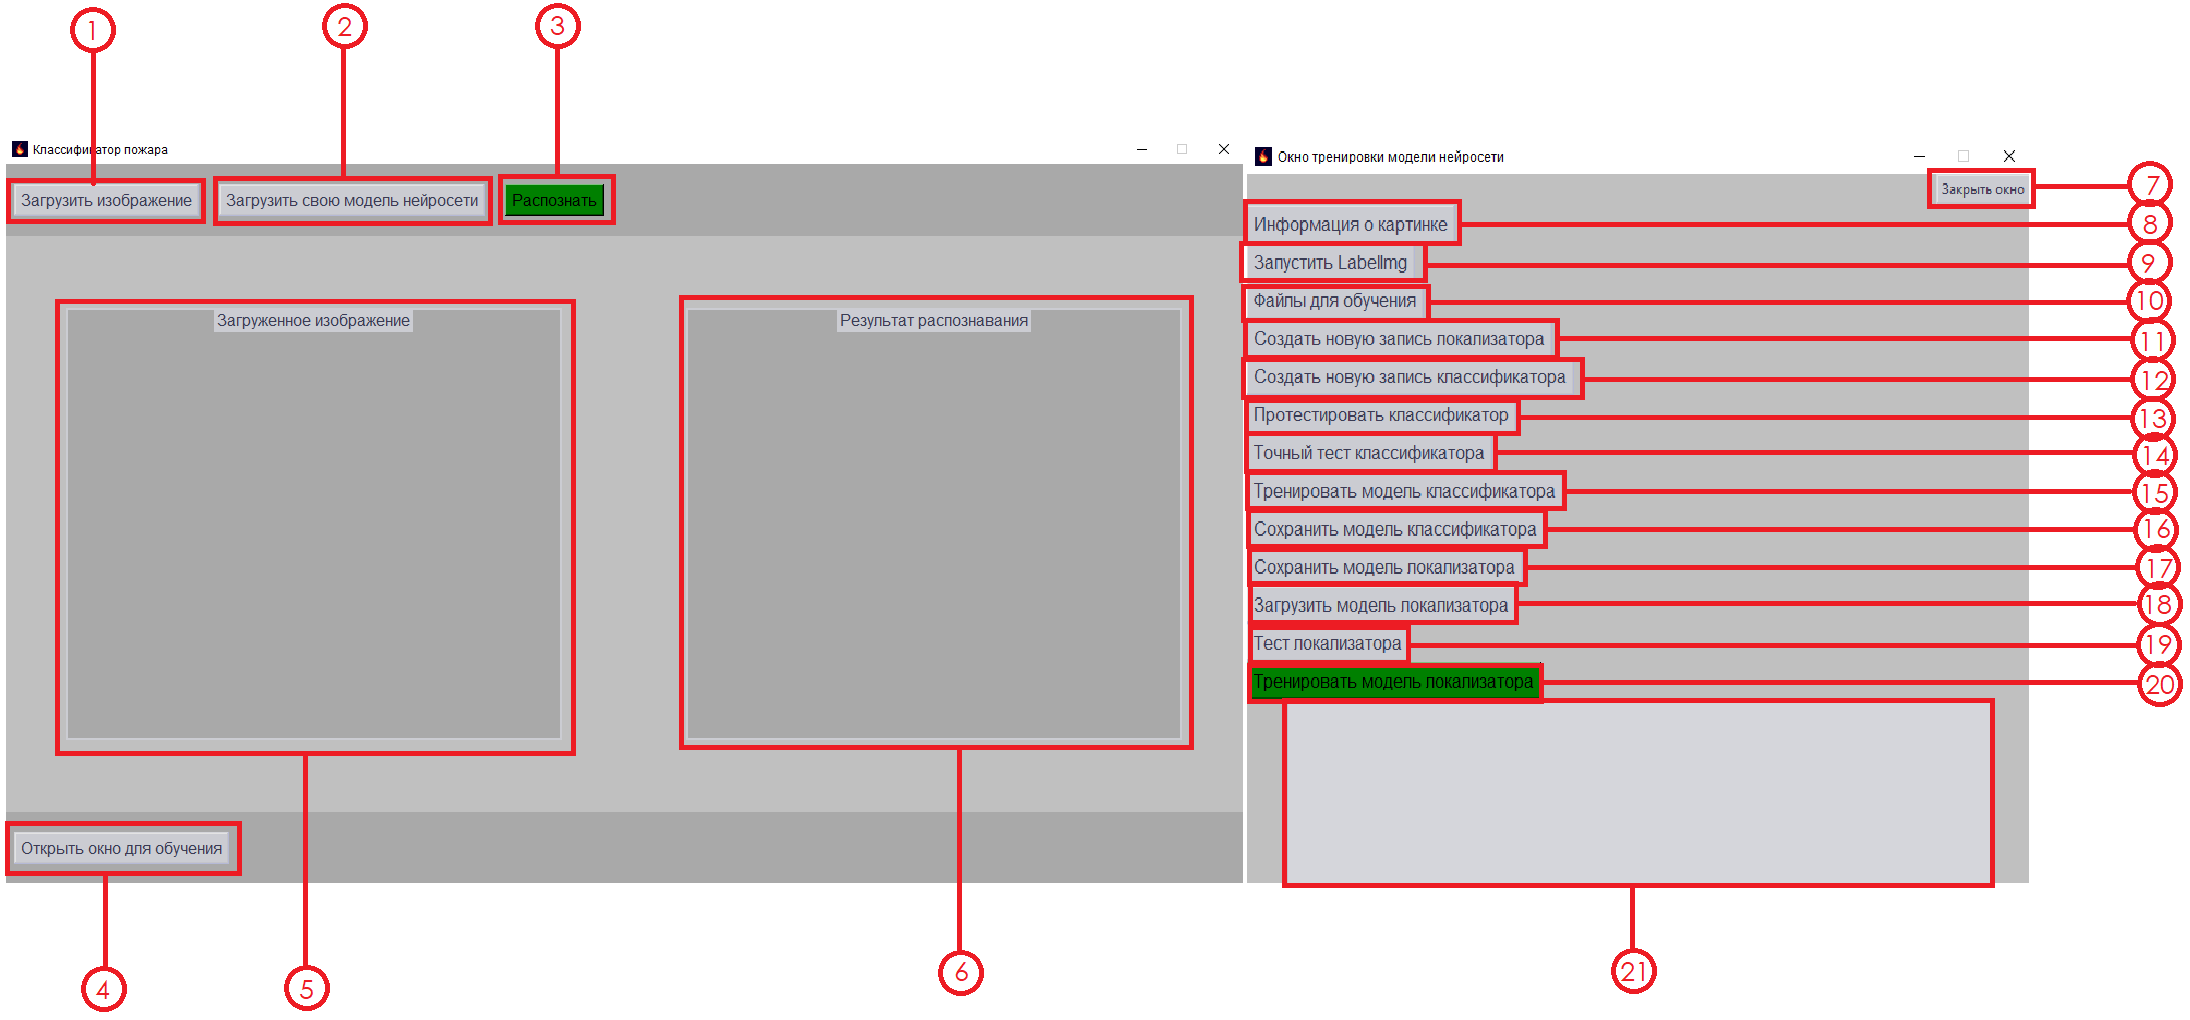
\includegraphics[width=1\linewidth]{maketinterface}}
\caption{Макет интерфейса окна распознавания и окна обучения нейронной сети}
\label{maketinterface:image}
\end{figure}
